\newpage
\section{Part D}
\label{sec:sec_d}
Next, the two fine and coarse classifiers were combined into a single class called \textit{BrainNet}. Which when given an inputs returns both the fine and coarse classification while sharing a common feature extractor to prevent redundant computations.  

\LST{part\_d}

In order to test out the \textit{BrainNet} model a non-\textit{CIFAR-100} dataset was chosen. The test data comes from the \textit{Tiny-ImageNet} dataset downloaded from \textit{Hugging Face}\footnote{https://huggingface.co/datasets/zh-plus/tiny-imagenet}. This dataset contained 100,000 64x64 images spread across 200 class labels. The images were resized and normalized to match the \textit{CIFAR-100} images used in training. Because this data is coming from a different dataset with different labels it wouldn't be expected the the \textit{BrainNet} model would get equal performance to the test set used in the previous sections. Additionally a large number of the \textit{Tiny-ImageNet} don't have a direct analogous \textit{CIFAR-100} label. To address this problem 11 classes were chosen from the \textit{Tiny-ImageNet} labels that either directly overlapped with \textit{CIFAR-100} labels or I determined were similar enough that the model should be able to classify them. The mapping of the chosen 11 classes is as follows, for the coarse labels they were chosen to be the corresponding coarse label to the associated fine label. 

\LST{part\_d\_2}

Using the chosen labels as a subset of the \textit{Tiny-ImageNet} dataset, there were 5440 new images that could be tested. After running them through the \textit{BrainNet} model (which was training on \textit{CIFAR-100} data), the model produced the accuracies shown in Table~\ref{table:bn acc}. As can be seen the model did quite well at classifying these new images. 

\begin{table}[h!]
	\centering
	\begin{tabular}{|c|c|c|}
		\toprule
		\textbf{BrainNet} & \textbf{Top-1} & \textbf{Top-5} \\
		\midrule
		Fine & 0.68 & 0.84 \\ \hline
		Coarse & 0.74 & 0.92 \\ \hline
	\end{tabular}
	\caption{\textit{BrainNet} Accuracies}
	\label{table:bn acc}
\end{table}

For further results the confusion matrix was generated for the coarse labels in Figure~\ref{fig:coarse cm}. As can be seen the biggest issue was with the images labeled, either \textit{snail} or \textit{lobster} by the \textit{Tiny-ImageNet} dataset. They were frequently confused with the \textit{CIFAR-100} coarse label \textit{insects}. It is easy to imagine how those could be challenging for the classifier. For completeness the fine classification confusion matrix is attached in Figure~\ref{fig:fine cm}, however due to the number of classes it is difficult to read.

\begin{figure}[h]
	\centering
	\includegraphics[width=\textwidth]{figures/coarse\_cm.png}
	\caption{Coarse Accuracies}
	\label{fig:coarse cm}
\end{figure}

Next we consider 100 randomly chosen images from the \textit{Tiny-ImageNet} dataset. The trail results are shown in Figure~\ref{fig:100 test}. From these 100 predictions, it was found that in the case of the coarse labels where teh model is correct the average confidence was 97.5\%, and 69.4\% when incorrect. For the fine model the average correct confidence was 99.2\% and 51.4\% when incorrect.

\begin{figure}[h]
	\centering
	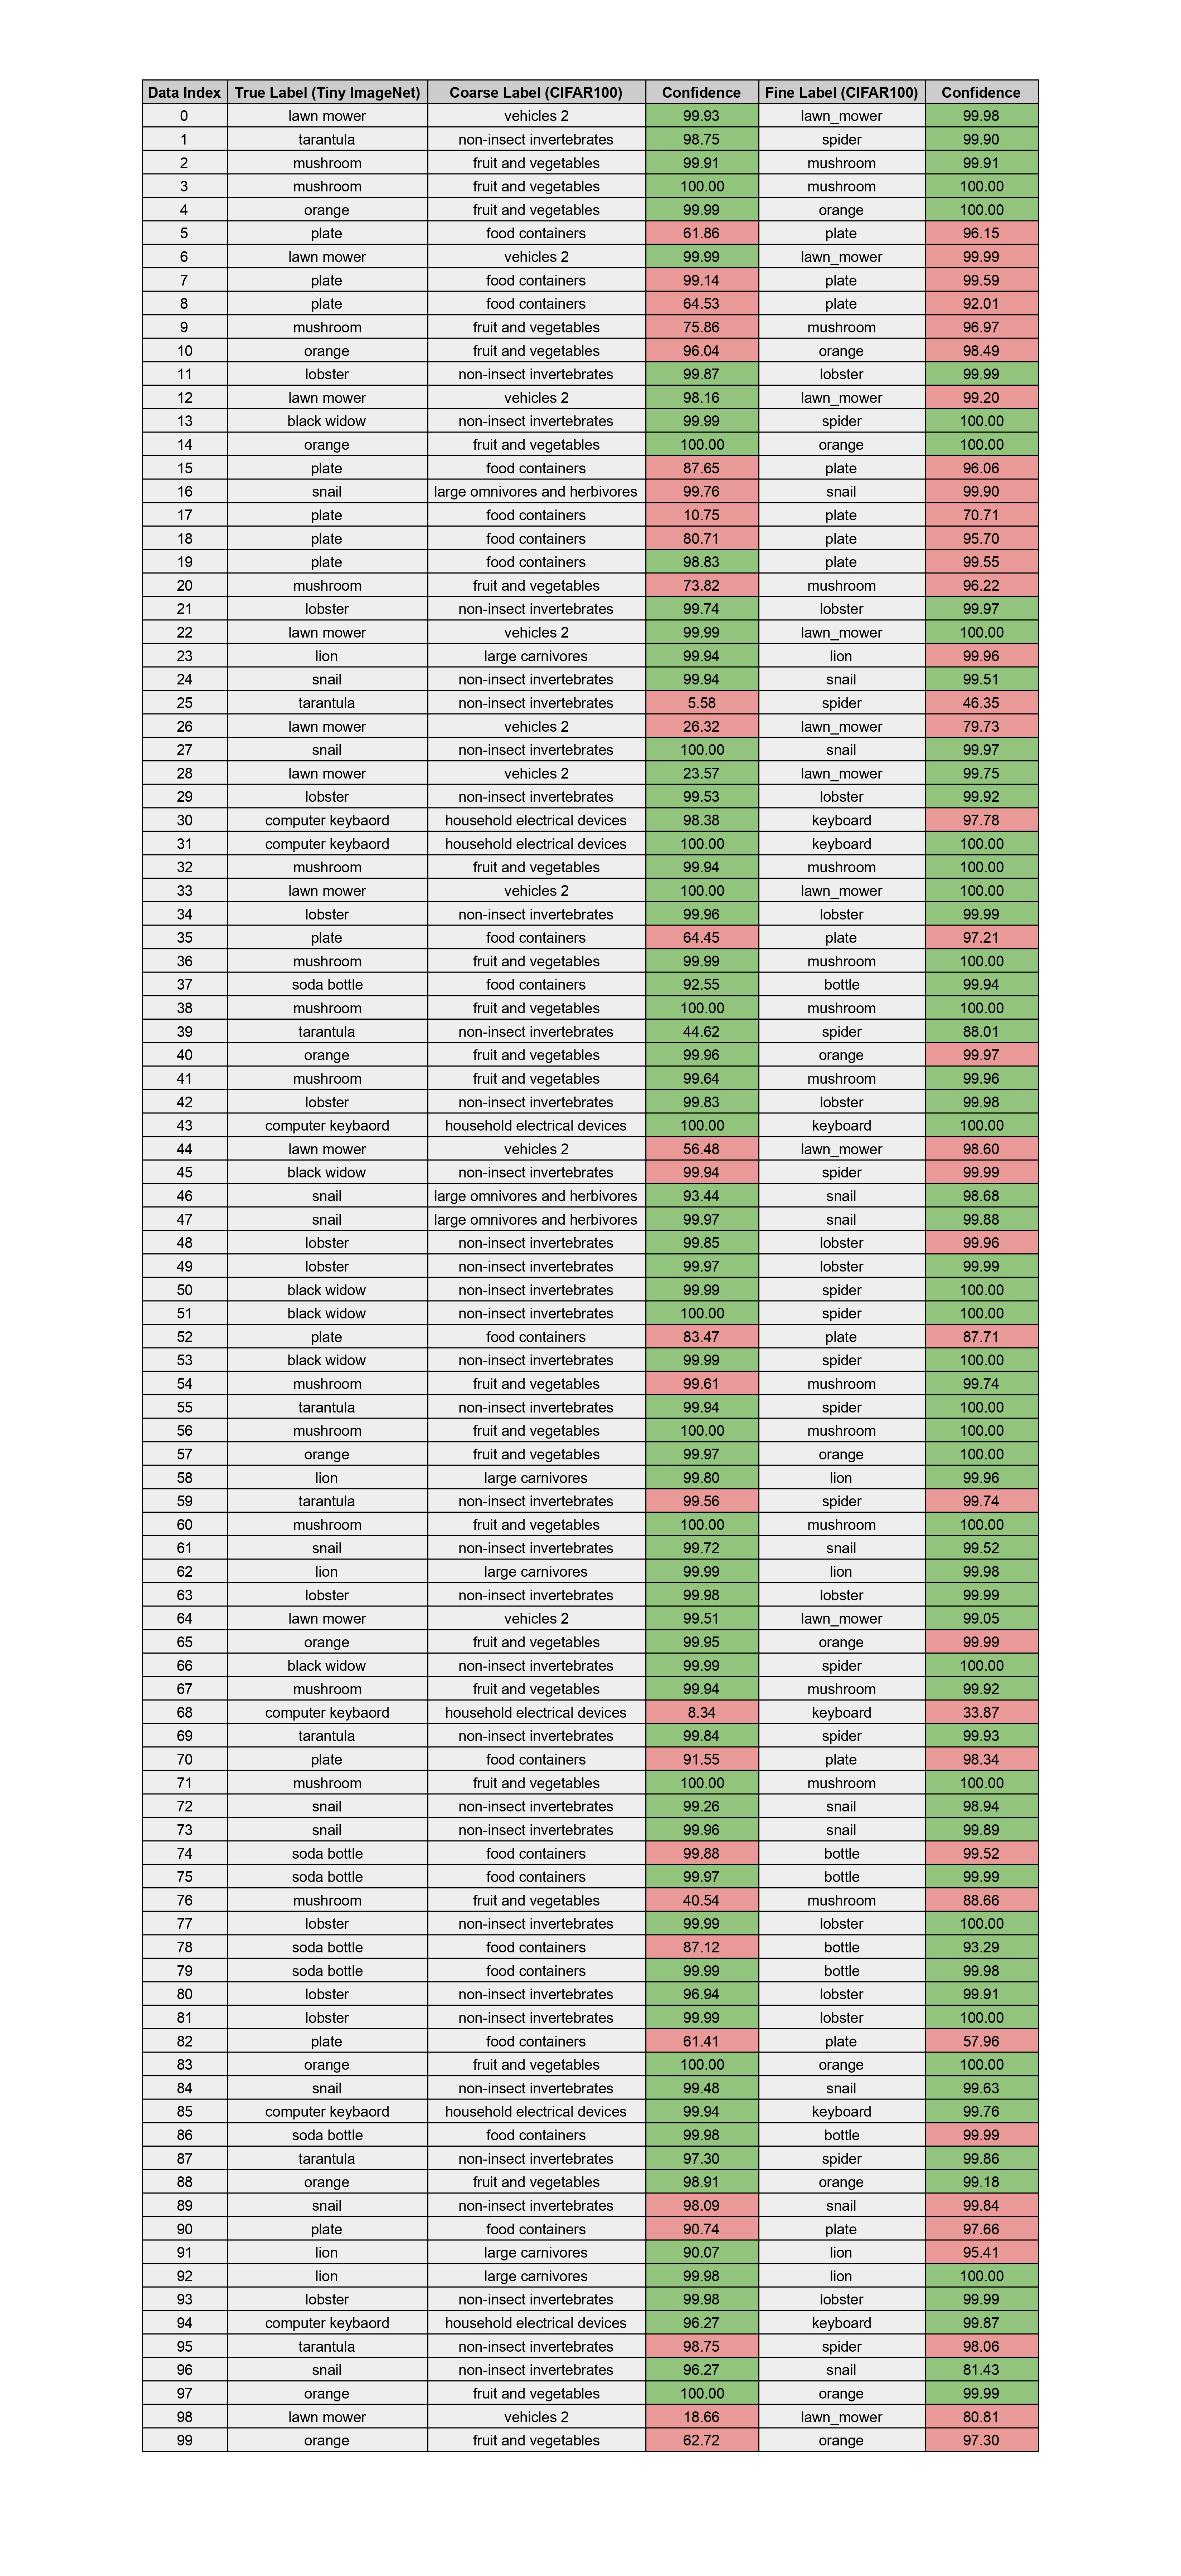
\includegraphics[height=\textheight]{figures/tiny-100.jpg}
	\caption{100 \textit{Tiny-ImageNet} Test Points}
	\label{fig:100 test}
\end{figure}

\begin{figure}[h]
	
	\centering
	\includegraphics[width=\textwidth]{figures/fine\_cm.png}
	\caption{Fine Accuracies}
	\label{fig:fine cm}
	
\end{figure}